\chapter{Results}

The last chapter of the thesis describes the experiments that were performed to~provide a clear result of the MHCA implementation performance. The aim of~the~thesis was to create the MHCA implementation that is capable of clustering datasets of hundred thousands and millions of points in a reasonable amount of~time.

The results were compared with a different implementation of Mahalanobis-based hierarchical clustering \cite{fivser2012detection}. It is a R language implementation with performance critical parts written in C language. It provides both FMD and CMD measures of dissimilarity and the apriori clusters computation as well. It performs a~serial CPU computation. For brevity, we denote the thesis GPU implementation by \texttt{gmhclust} and the serial CPU version by \texttt{mhclust}.

The testing datasets were divided into these two categories:

\begin{description}
	\item[Single-point datasets] These datasets are clustered without a knowledge of any apriori clusters. Hence, the computing starts from a single point. The datasets are purely of a high-dimensional flow and mass cytometry data \cite{flowrepo} (see tab.~\ref{tab04:single}).
	
	\begin{table}
		\centering
		\begin{tabular}{lcc}
			\toprule
			\textbf{Dataset name} & \textbf{Size} & \textbf{Dimension} \\ \midrule
			\emph{Niellson\_rare} &      44K      &         14         \\
			\emph{Levine\_13dim}  &     167K      &         13         \\
			\emph{Levine\_32dim}  &     265K      &         32         \\
			\emph{Mosmann\_rare}  &     396K      &         15         \\
			\emph{Samusik\_all}   &     841K      &         39         \\ \bottomrule
		\end{tabular}
	\caption{Flow and mass cytometry datasets selected for experiments.}
	\label{tab04:single}
	\end{table}

	\item[Apriori datasets] These datasets are clustered with apriori clusters. They do not represent any measured data. Rather, for each dataset, a set of distinct clusters was artificially created for this purpose. Each cluster was randomly generated as a set of $d$-dimensional points with the normal distribution and evenly scattered among the dataset. The describing parameters of~apriori datasets are the \emph{apriori cluster size}, the \emph{apriori cluster count} and the \emph{point dimensionality} (see tab.~\ref{tab04:apriori}). To find the apriori clusters, they need not be pre-computed by another clustering algorithm (such as k-means) as~all the~points are already stored with respect to the apriori clusters.
	
	\begin{table}
		\centering
		\begin{tabular}{lcccc}
			\toprule
			\textbf{Dataset name} & \textbf{Cluster size} & \textbf{Cluster count} & \textbf{Size} & \textbf{Dimension} \\ \midrule
			\emph{apriori\_1M}    &         1000          &          1000          &      1M       &         20         \\
			\emph{apriori\_2M}    &         2000          &          1000          &      2M       &         20         \\ \bottomrule
		\end{tabular}
		\caption{Apriori datasets generated for experiments.}
		\label{tab04:apriori}
	\end{table}
	
\end{description}

All experiments were run on the same machine (Intel Xeon Silver 4110, 256 GB RAM, NVIDIA Tesla V100 PCIe 16 GB). The performance related experiments were performed several times. As there were negligible performance differences in the separate runs, all the following plots depicting performance show their arithmetic means. 

\section{The closest neighbor parameter}

To determine which clusters to merge, the GPU implementation uses the closest neighbor array. The number of the closest neighbors assigned to each cluster in~the~array is variable. We experimented on single-point and apriori datasets with this parameter to determine which number performs best. 

We assumed that \emph{two} closest neighbors will achieve the best performance as~it will result in the reduced number of cluster to be updated each iteration. \emph{Three} and more neighbors will not provide such reduction that would compensate the~diminishing returns caused by the longer time for a cluster update.

\begin{figure}\centering
	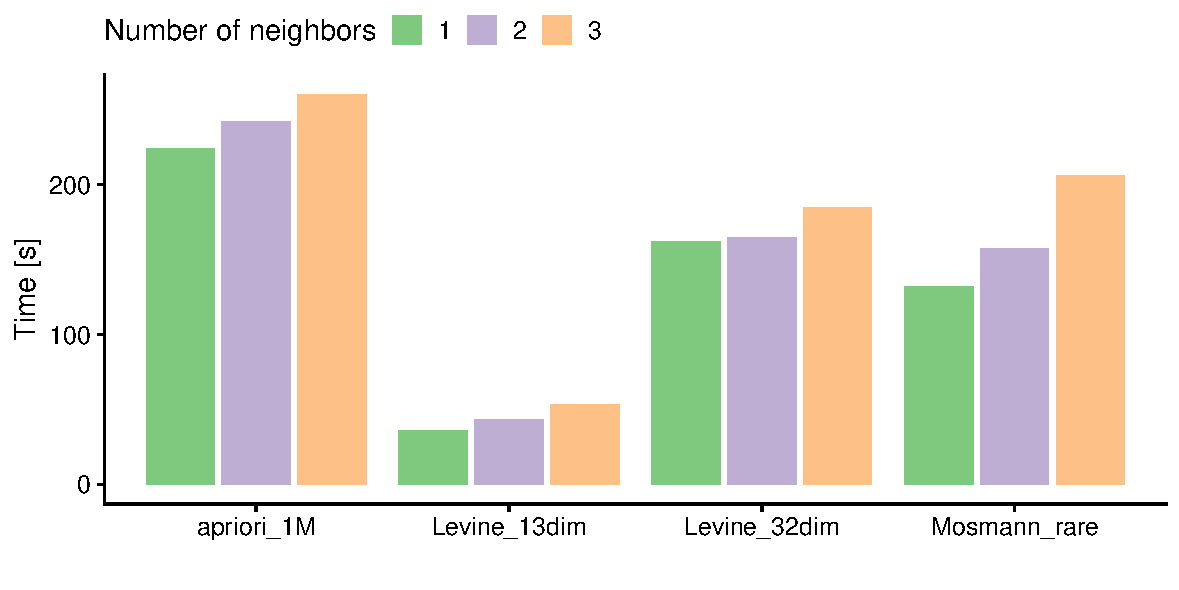
\includegraphics[width=\linewidth]{img/neighbor_compare}
	\caption{A comparison of \texttt{gmhclust} with various numbers of neighbors assigned to clusters.}
	\label{fig04:neigh}
\end{figure}

As can be seen from the figure \ref{fig04:neigh}, the variant of 1 closest neighbor achieved the~best performance. It may be caused by the fact that the lower number of cluster updates did not overcome the increased time for each update. Alternatively, it may be caused by the composition of tested datasets; datasets that naturally form cluster of other than elliptical shape may benefit better from another closest neighbor number variant.

The forthcoming experiments will be performed with the 1 closest neighbor variant.

\section{Performance speedup}

The next set of experiments determines the performance speedup of~the~GPU implementation over the CPU implementation. The performance comparison was performed on single-point and apriori datasets separately.

Unfortunately, during the single-point testing, we reached the computational limits of the CPU implementation. Even for the smallest dataset, the computation took nearly 14 hours. Due to the polynomial time complexity and extremely increasing memory requirements (193GB for Levine\_32), we decided that in order to test the datasets, we need to down-sample them. We uniformly randomly selected a fraction of the dataset points to create a smaller dataset. Note that these consequences are necessary (yet unforeseen) as the larger datasets require such big amount of time and space resources that they are by no means practically computable (see fig.~\ref{fig04:fract_comp}).

\begin{figure}\centering
	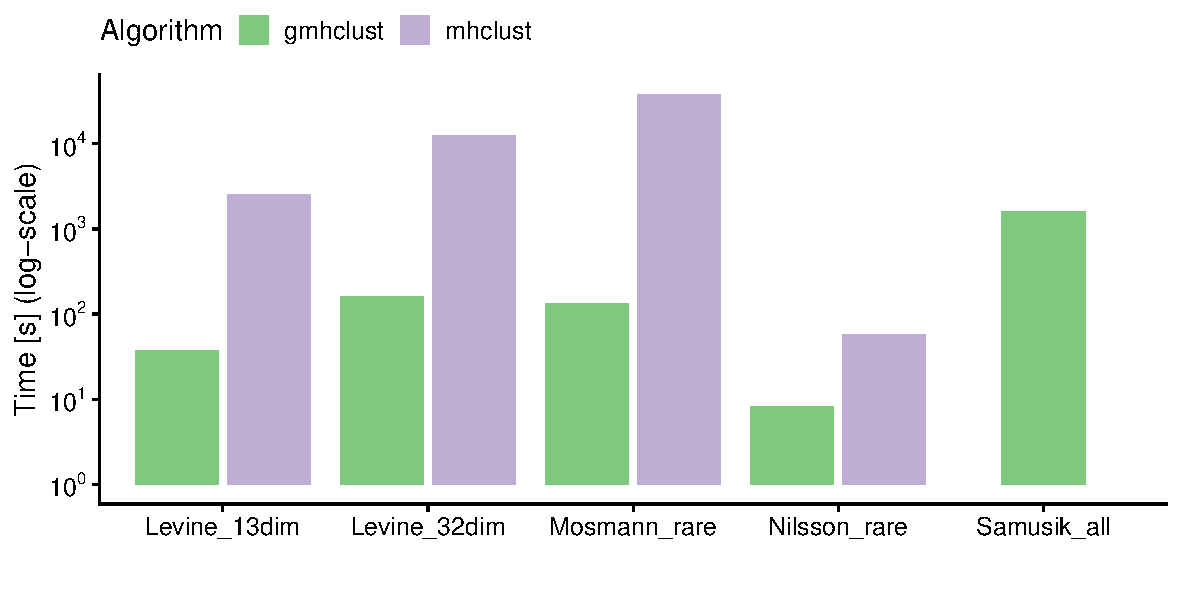
\includegraphics[width=\linewidth]{img/mixed_perf_comp}
	\caption{An example of a poor performance of \texttt{mhclust} compared with \texttt{gmhclust} on single-point datasets. Datasets of \texttt{mhclust} were down-sampled to the fraction of $\frac{1}{10}$ while \texttt{gmhclust} datasets were not changed. For Samusik\_all dataset, neither the fraction of $\frac{1}{10}$ did help to finish the computation within a 24 hours mark.}
	\label{fig04:fract_comp}
\end{figure}

\subsection{Single-point datasets performance speedup}

To determine the performance increase, we decided to down-sample Nillson\_rare dataset (as it is the smallest one). We created 10 samples with their sizes corresponding to 10\% of the dataset up to 100\%.
As seen from the figure \ref{fig04:single_perf}, the~performance difference increases as the~dataset size increases. It is a common consequence of~the~fact that there is less work to parallelize in smaller datasets than in~bigger datasets. In the dataset of size around 4K, the performance of \texttt{gmhclust} is 60-times greater. This scales up to 5000-times faster time for the full Nilsson\_rare dataset.

\begin{figure}\centering
	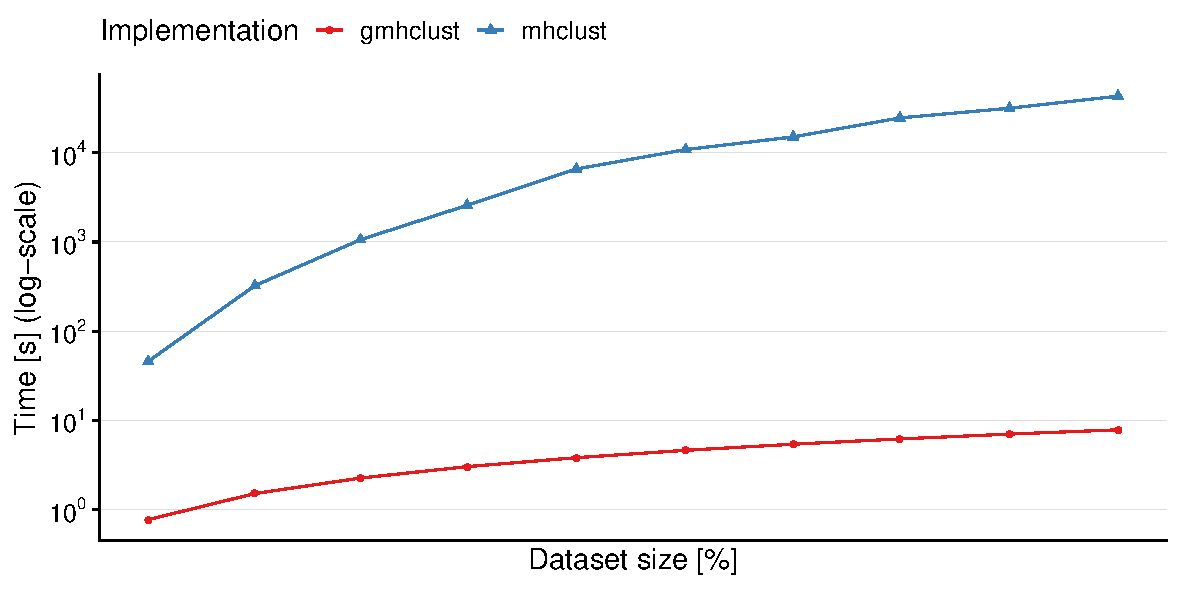
\includegraphics[width=\linewidth]{img/single_perf_comp}
	\caption{A comparison of \texttt{gmhclust} and \texttt{mhclust} performance on various sizes of Nilsson\_rare single-point dataset.}
	\label{fig04:single_perf}
\end{figure}

\subsection{Apriori datasets performance speedup}

In contrast with the single-point datasets, the CPU implementation managed to~compute apriori datasets of big sizes. It is a consequence of the wisely chosen apriori clusters.

When the algorithm is inputed with apriori clusters, it does not compute the~whole dataset at once --- it clusters each apriori cluster first. This fact reduces the overall time complexity significantly, allowing the CPU algorithm to compute big datasets in a short amount of time.

For example, suppose the input dataset apriori\_2M and a function $f$ that takes a dataset size and outputs the required time for its clustering. Then, the algorithm performance is proportional to $$1000f(2000)+f(1000)$$ that is --- deducing from the previous experiment --- far less than $f(1000\cdot 2000)$.

We measured the performance of the CPU and GPU implementation on apriori\_1M and apriori\_2M (see fig.~\ref{fig04:apr_perf_comp}). The results of the performance increase are~8-times and 20-times respectively. As we expected, it is not as measurable as~in~single-point datasets even though it has much more points. 

It is caused by computing a lot of small apriori clusters. From the previous experiment we observed that small-sized datasets do not exhibit such big increase in performance. Therefore, the overall performance increase in apriori datasets is not expected to be drastically better.

\begin{figure}\centering
	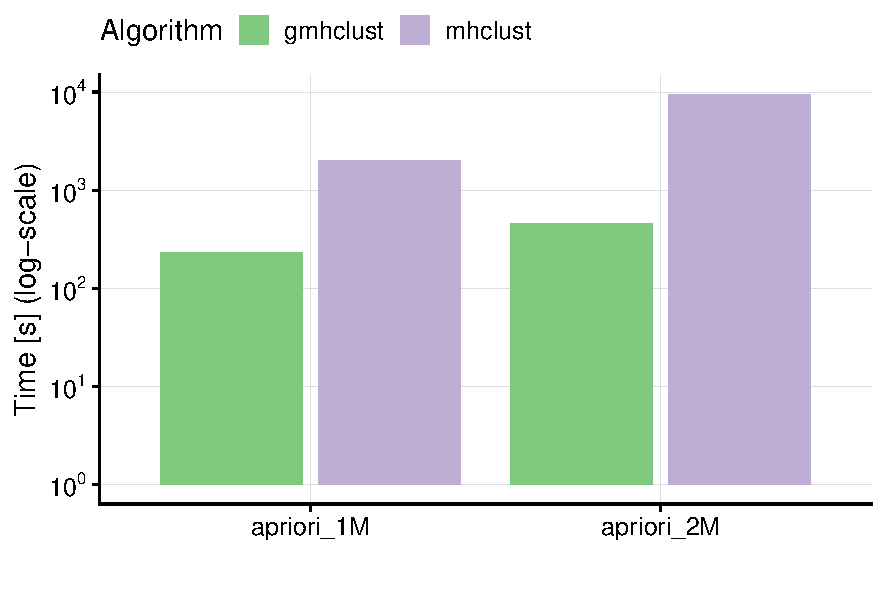
\includegraphics[width=10cm]{img/apriori_perf_comp}
	\caption{A comparison of \texttt{gmhclust} and \texttt{mhclust} on apriori datasets.}
	\label{fig04:apr_perf_comp}
\end{figure}

\subsubsection{Apriori dataset parameters}

The next experiment tests how the apriori dataset parameters \emph{size} and \emph{count} influence the overall algorithm time. We tested 7 different size--count ratios on~a~dataset of~5M 20-dimensional points (see fig.~\ref{fig04:apr_ratio}). The Mahalanobis threshold of each run was set to be equal to the apriori cluster size.

The runs are ordered in such way that the apriori cluster size is increasing (and the apriori cluster count is decreasing). The plotted line first rapidly decreases, then is close to constant and starts to increase in the end. This may be~caused by two factors:

First, according to the previous experiment, we expected the following relation: the bigger is the maximum of the size and count parameters, the bigger is~the~overall computational time. Hence, big measured values are seen on~the~edges of the plot. 

The second factor may be the Mahalanobis threshold. As the threshold increases with the increasing cluster size, more clustering work is performed using the less demanding euclidean distance. The threshold was set to be equal to~the~apriori cluster size; hence, the Mahalanobis distance is used after all apriori clusters are clustered. As the consequence, the right edge of the plot is~not as~steep as the left edge.

\begin{figure}\centering
	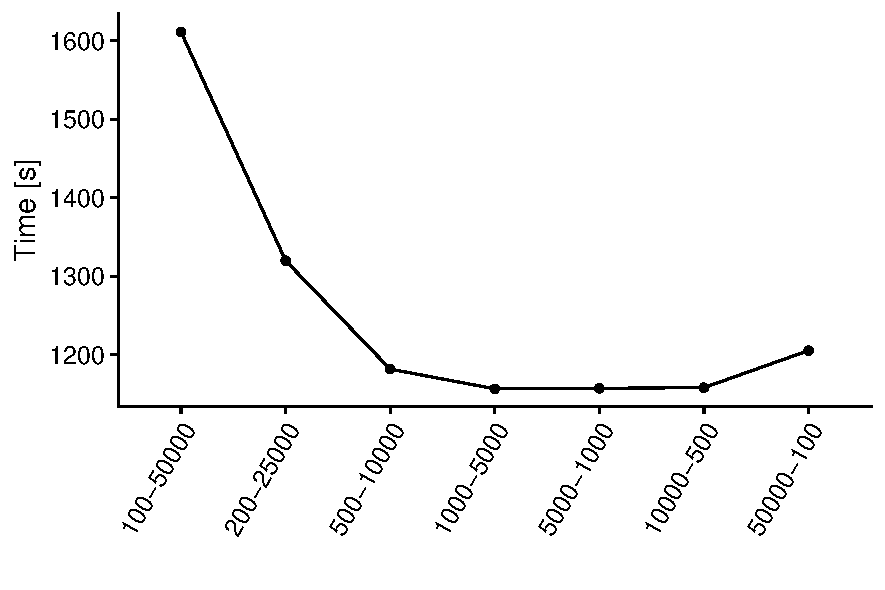
\includegraphics[width=10cm]{img/5M-compare}
	\caption{\texttt{gmhclust} performance for different ratios of apriori cluster size and count (depicted as $size$-$count$) with Mahalanobis threshold set to $size$.}
	\label{fig04:apr_ratio}
\end{figure}

\section{Results comparison}

Next, we will compare the clustering results of the GPU and CPU implementation to see if they are similar. Comparing results for equality would put big restrains on the implementation. Rather, we want to allow algorithms to have slight differences during their clustering and compare the whole clustering process. First, we need to define the \emph{point height}.

\begin{defn}[Point height]
	Suppose a dataset $\mathcal{D} \subset \R^d$  and an ordered sequence of cluster pairs $p_1,\dots,p_{n-1}$ that defines a result $\mathcal{R}$ of a hierarchical clustering on~$\mathcal{D}$. We define the \emph{height of point} $o \in \mathcal{D}$ in $\mathcal{R}$ as the sum of distances between all cluster pairs $p_i$ such that $o$ belongs to  their union.
\end{defn}

We can easily imagine point height using a dendrogram. The point height represents the distance from the bottom of the dendrogram (starting in the~corresponding point) to the top.

To compare two clusterings, we compute the height of each point in both clusterings. Then we take the two distances of each point as its coordinates and put them on the two-dimensional plane. If they create a straight increasing line, it means that the correlation between point heights of two clusterings is equal to~1 and that clusterings formed very similar clusters. When points are scattered among the whole plane, different clusters were created and the overall clusterings differ.

An another approach for comparing hierarchical clusterings is to compare a selected parts of their dendrograms. Dendrograms are \emph{cut} to expose a small amount of clusters (i.e.~10). Then, they are directly compared using similarity measures like the F-score.

However, a MHCA algorithm tends to create small clusters that are propagated to~the~very top of the dendrogram. They usually consist of noise; Mahalanobis distance makes them dissimilar to the rest and they are merged in the late clustering stages. This can be a problem for the direct cluster comparison as these noise clusters can easily skew the results. In compared clusterings, they may be composed of different points or form different amount of cluster; all this can worsen the result of potentially similar clusterings. 

Hence, we preferred the first method for comparing two clusterings as it takes the whole dendrogram into the account rather than a selected part.

\subsection{Single-point dataset results comparison}

We down-sampled four selected single-point datasets to the fraction of $\frac{1}{10}$. Then, we computed heights of each point and plotted them as discussed above (see fig.~\ref{fig04:single_result}). The figure shows, that that GPU implementation chose different paths during its clustering process creating a different result. However, we can see that the points reside mainly on the diagonal; hence, the compared clusterings may created a lot of clusters that shared the majority of their points.

The possible reason of this behavior may be a slight difference in the measure of dissimilarity of the CPU implementation. There, small clusters are assigned an artificial covariance matrix so Mahalanobis distance can be applied on them. However, the GPU implementation computes only the euclidean distance. This can be a reason for branching of the algorithms in theirs early stages. As a consequence, the GPU and CPU clustering results differ slightly.

\begin{figure}\centering
	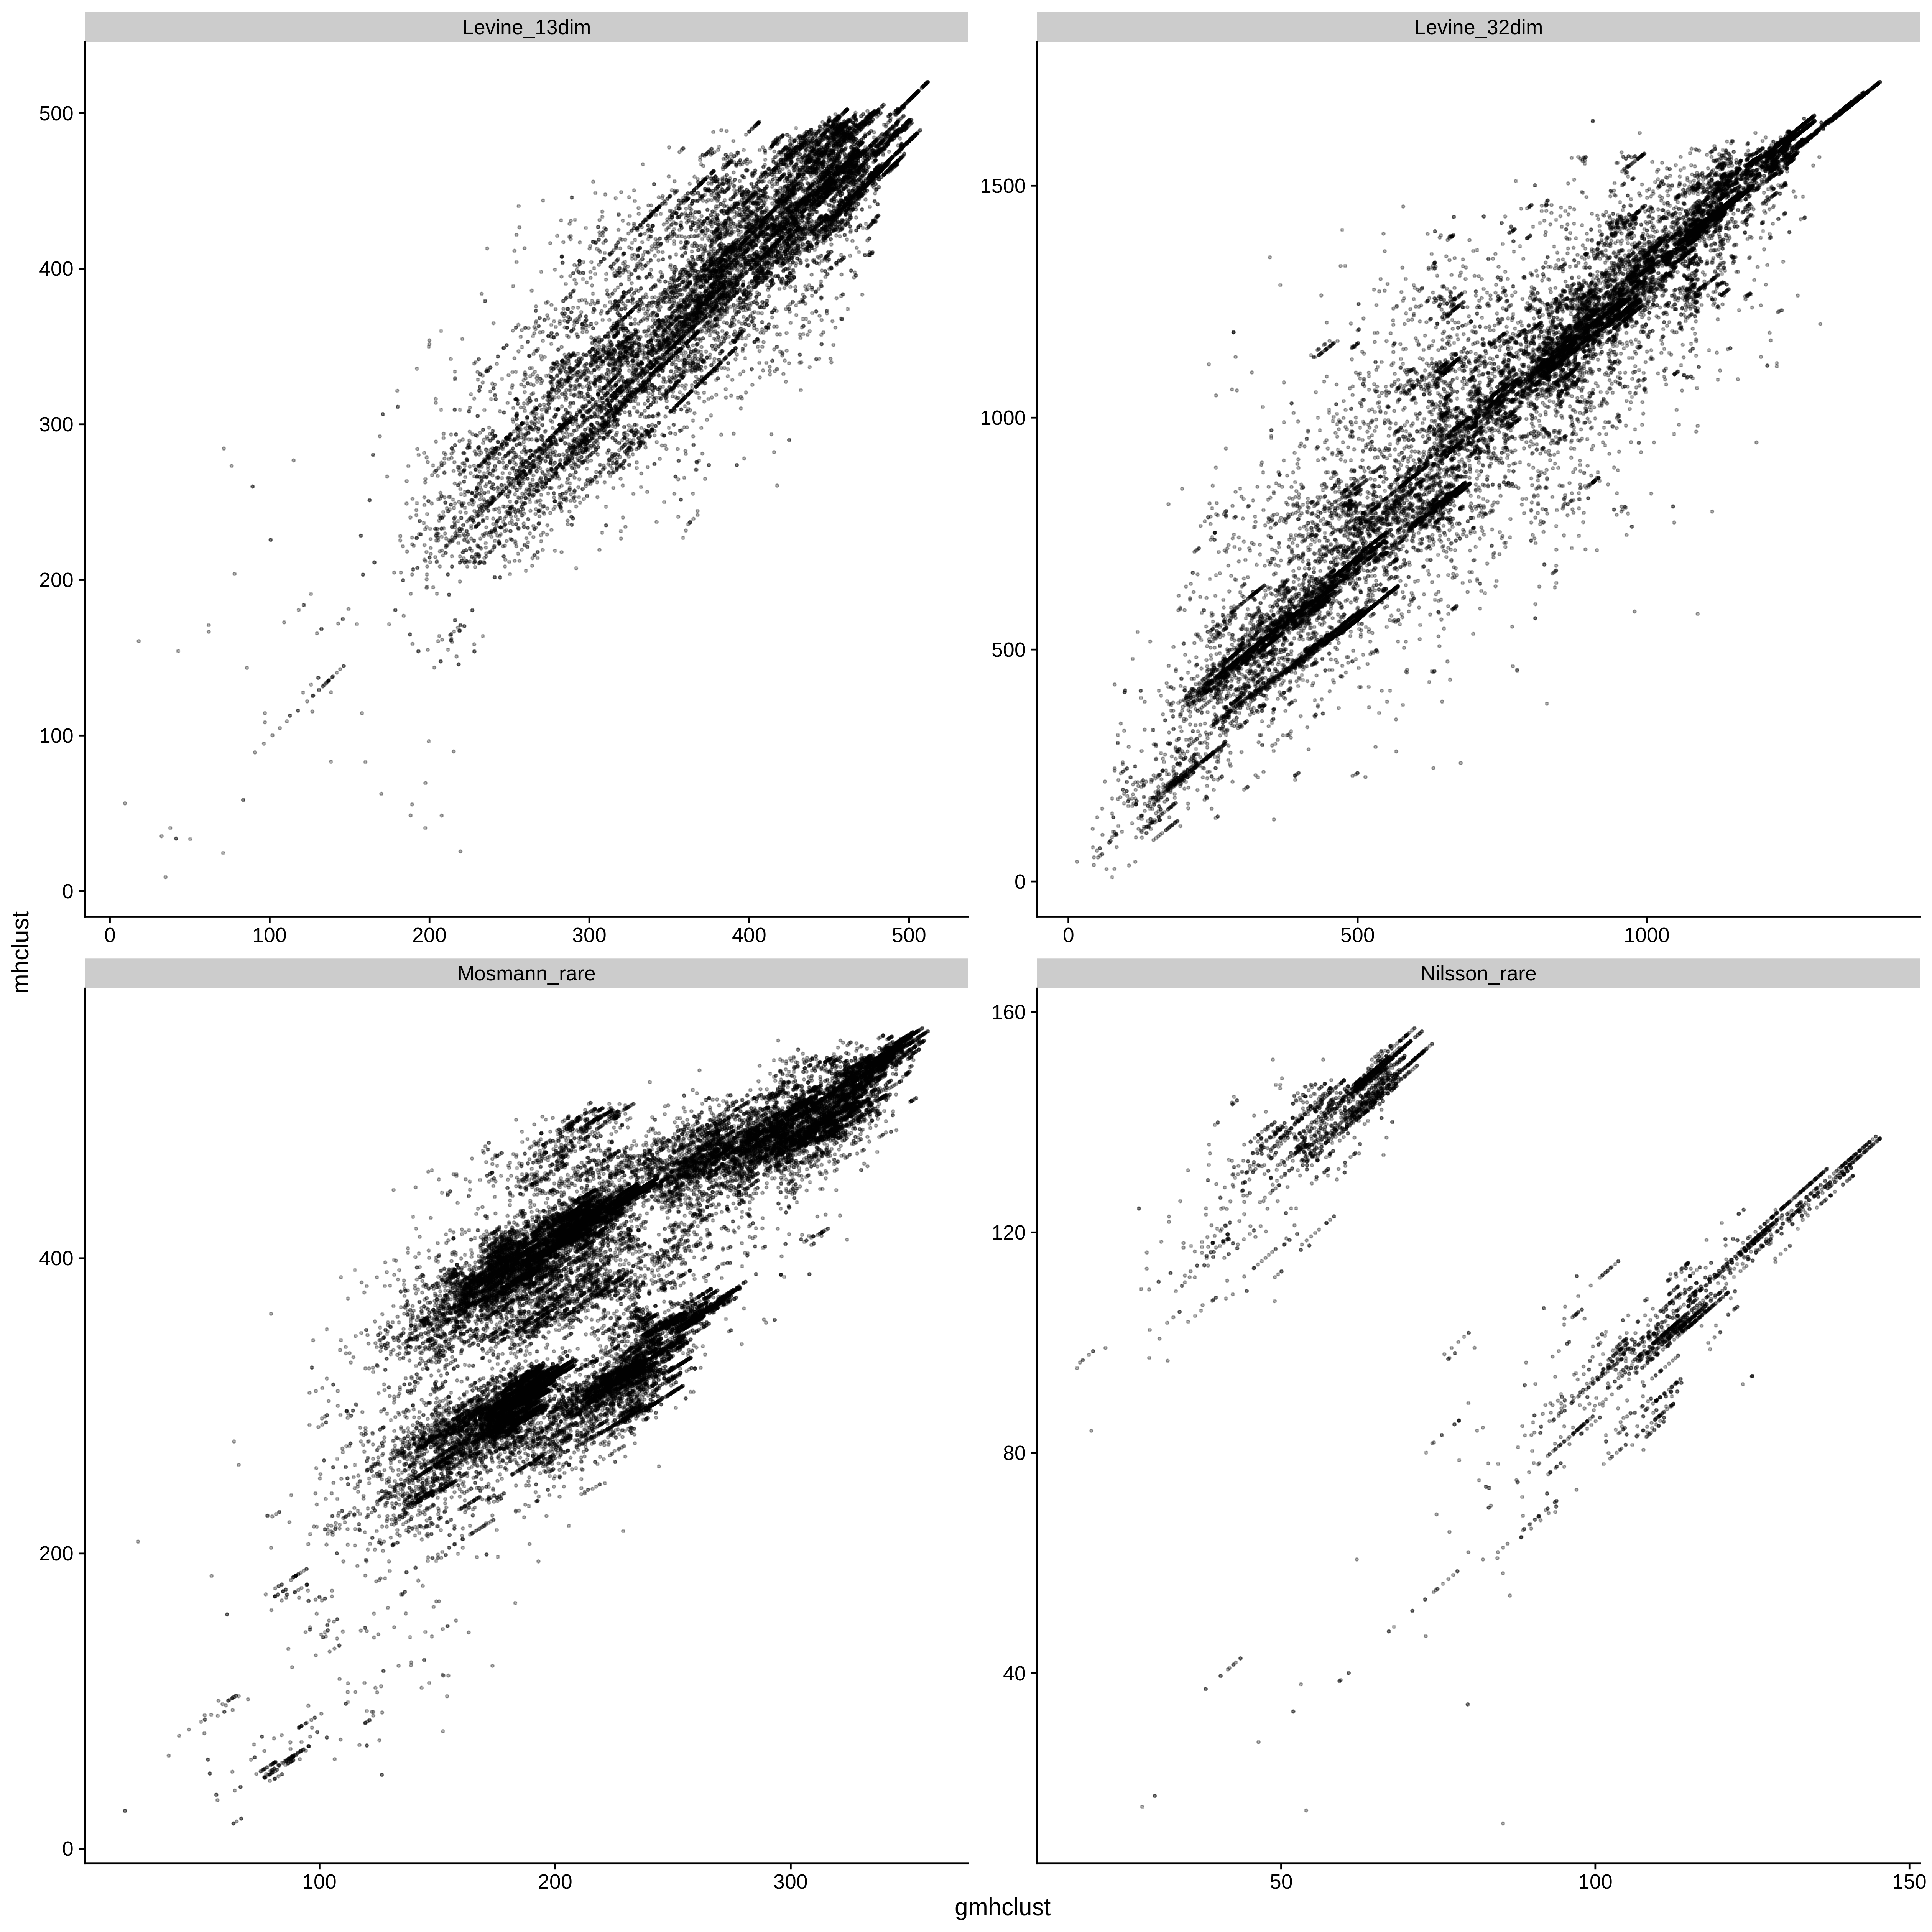
\includegraphics[width=\linewidth]{img/single_result}
	\caption{Plotted point heights of \texttt{gmhclust} and \texttt{mhclust} clusterings of~the~selected single-point datasets. The Mahalanobis threshold was set to default ($\frac{1}{2}$).}
	\label{fig04:single_result}
\end{figure}

\subsection{Apriori dataset results comparison}

We did not down-sample the selected apriori datasets and proceeded the same way as in the previous experiment (see fig.~\ref{fig04:apriori_result}). Here, the experiments showed the~almost straight line. It was expected, as the presence of apriori clusters effectively removed a possible error created during the early algorithm stages where the~implementations differed. More specifically, the propagation of possible clustering differences was stopped when the apriori clusters were completely clustered (as the clusterings aligned at that point).

When all apriori clusters were processed, the GPU and CPU measures of dissimilarity applied on the remaining clusters did not differ as the clusters were big enough. Hence, no other opportunity for possible branching occurred. This experiment also shows the importance of clustering early stages and how it can affect the~whole result.

\begin{figure}\centering
	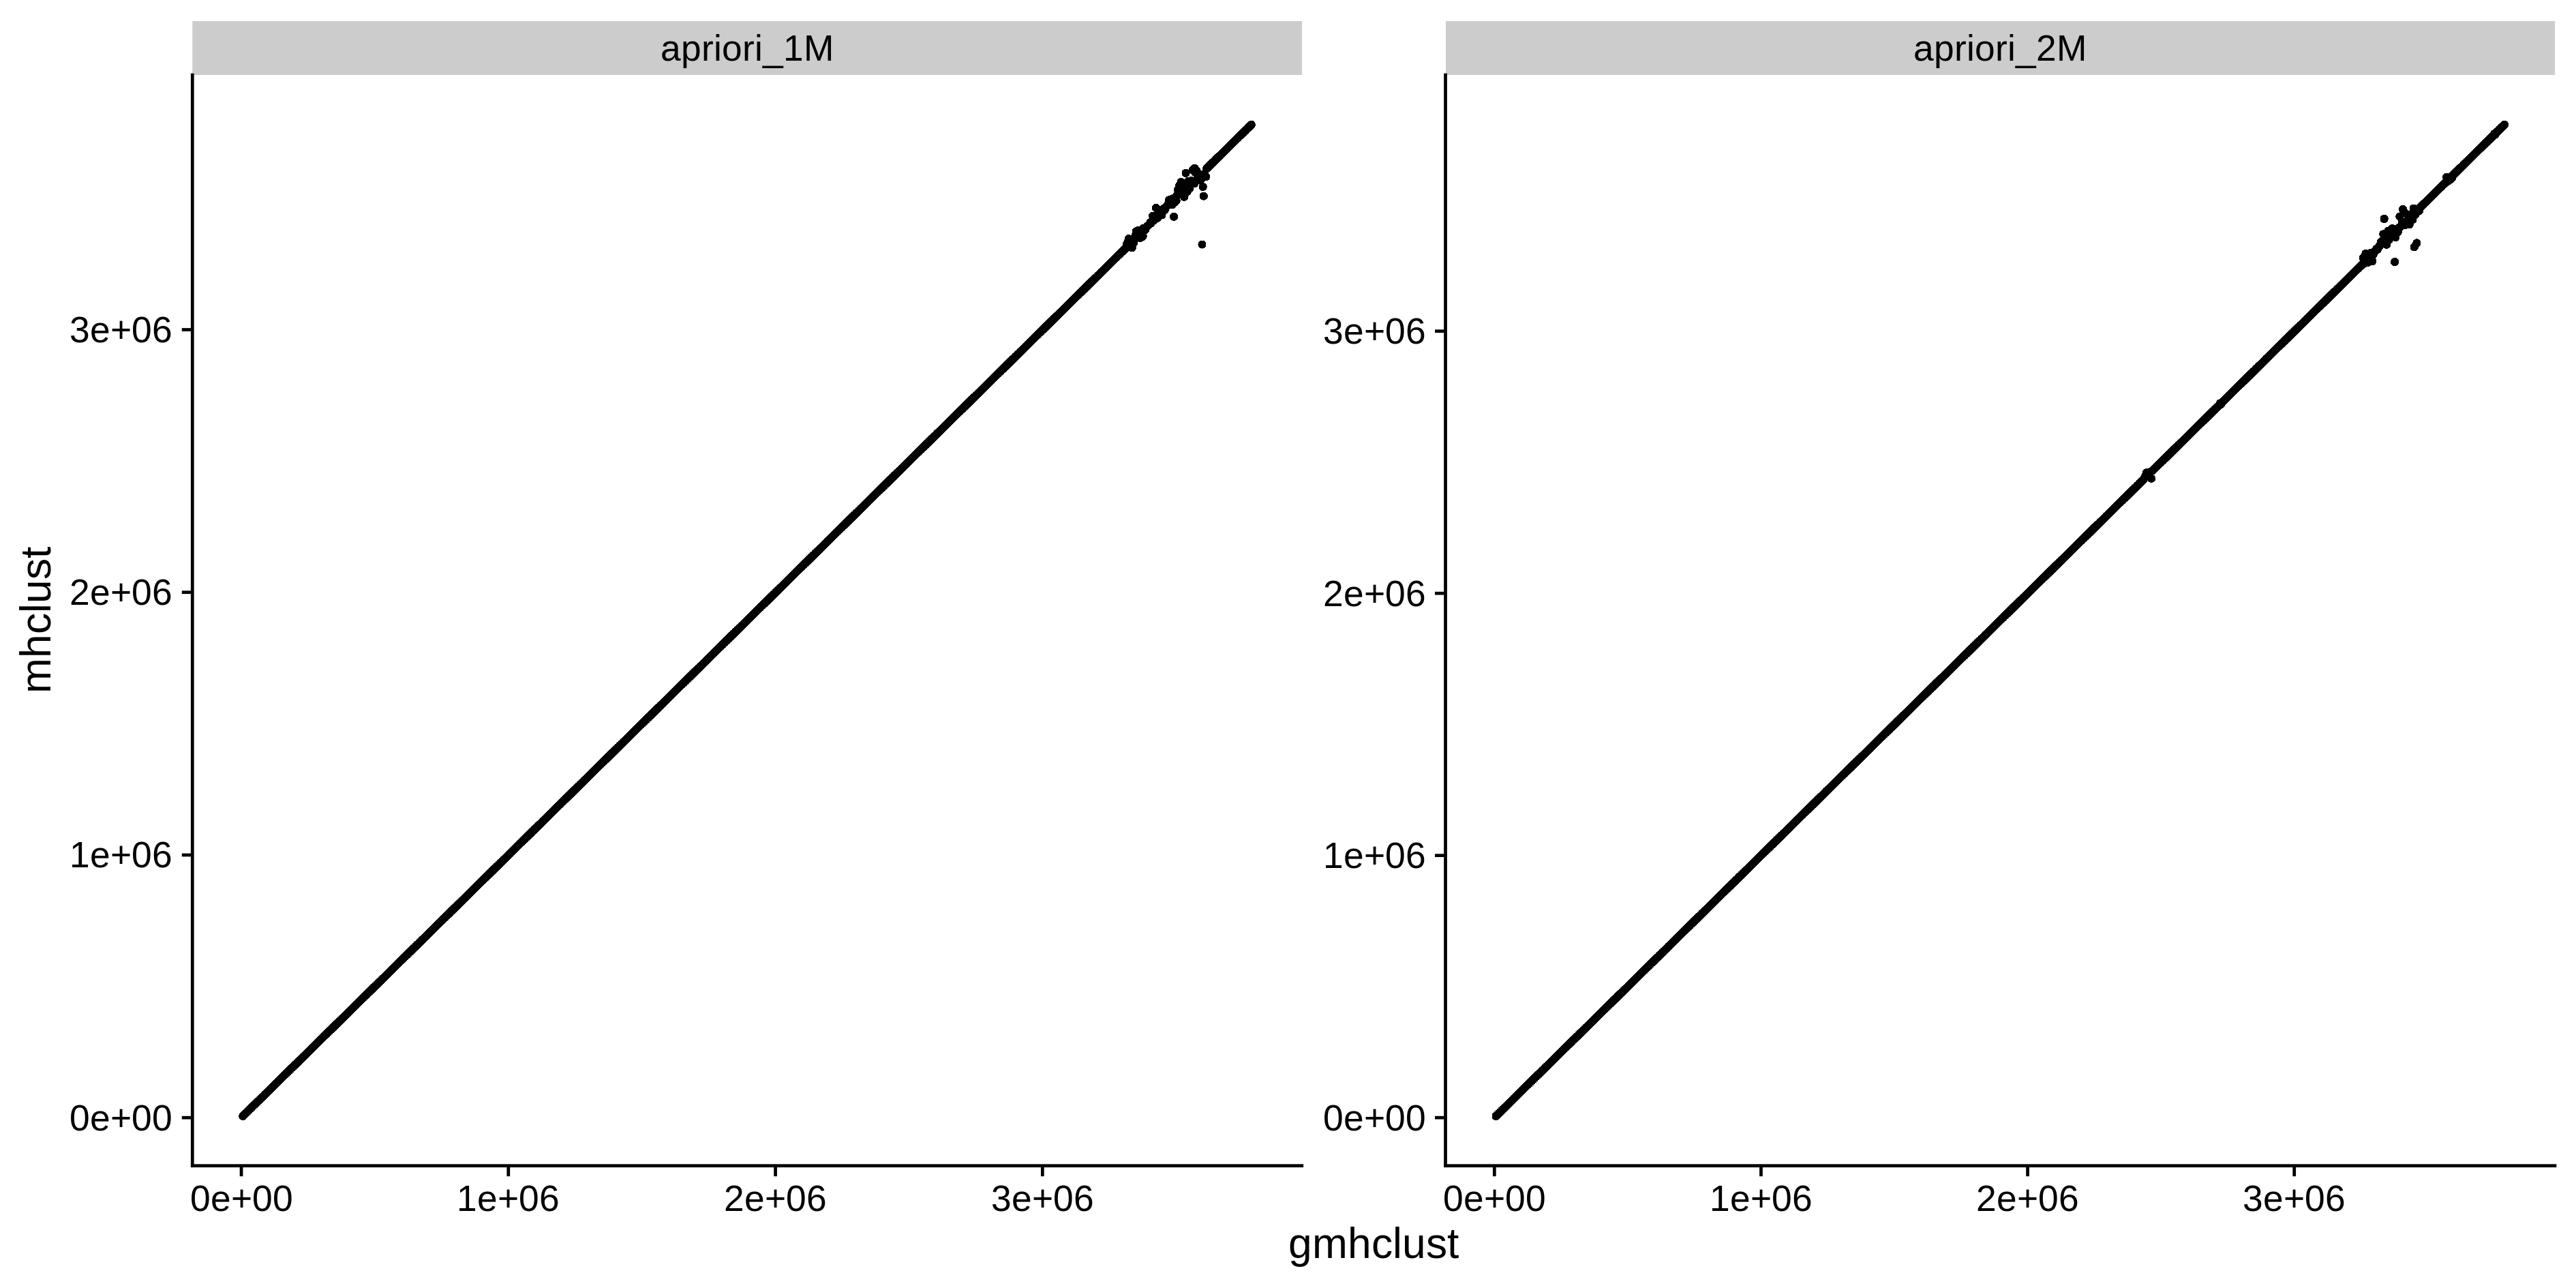
\includegraphics[width=\linewidth]{img/apriori_result}
	\caption{Plotted point heights of \texttt{gmhclust} and \texttt{mhclust} clusterings of~the~selected apriori datasets. The Mahalanobis threshold was set to apriori cluster size.}
	\label{fig04:apriori_result}
\end{figure}

